\documentclass[runningheads]{llncs}

\usepackage{cite}
\usepackage{amsmath,amssymb,amsfonts}
\allowdisplaybreaks
\usepackage{algorithm}
\usepackage{algorithmic}
\usepackage{graphicx}
\usepackage{textcomp}
\usepackage{xcolor}
\usepackage{booktabs}
\usepackage{rotating}
\usepackage{microtype}
\usepackage{url}
\usepackage{hyperref}
\usepackage{tikz}
\usetikzlibrary{shapes.geometric,arrows.meta,positioning,fit,backgrounds,calc}

\hypersetup{
    colorlinks=true,
    linkcolor=black,
    citecolor=black,
    urlcolor=black
}

% llncs predefines several theorem envs; define only the missing ones
\ifcsname definition\endcsname\else\newtheorem{definition}{Definition}\fi
\ifcsname axiom\endcsname\else\newtheorem{axiom}{Axiom}\fi
\ifcsname theorem\endcsname\else\newtheorem{theorem}{Theorem}\fi
\ifcsname proposition\endcsname\else\newtheorem{proposition}{Proposition}\fi
\ifcsname hypothesis\endcsname\else\newtheorem{hypothesis}{Hypothesis}\fi

\def\BibTeX{{\rm B\kern-.05em{\sc i\kern-.025em b}\kern-.08em
    T\kern-.1667em\lower.7ex\hbox{E}\kern-.125emX}}

\setlength{\textfloatsep}{6pt plus 1pt minus 2pt}
\setlength{\floatsep}{4pt plus 1pt minus 1pt}
\setlength{\dbltextfloatsep}{5pt plus 1pt minus 2pt}
\setlength{\dblfloatsep}{4pt plus 1pt minus 1pt}
\setlength{\abovecaptionskip}{3pt plus 1pt minus 1pt}
\setlength{\belowcaptionskip}{2pt plus 1pt minus 1pt}
\setlength{\abovedisplayskip}{3.5pt plus 1pt minus 1pt}
\setlength{\belowdisplayskip}{3.5pt plus 1pt minus 1pt}
\setlength{\abovedisplayshortskip}{1.5pt plus 1pt}
\setlength{\belowdisplayshortskip}{1.5pt plus 1pt}
\setcounter{dbltopnumber}{2}
\renewcommand{\dbltopfraction}{0.95}
\renewcommand{\dblfloatpagefraction}{0.85}

\begin{document}
\title{SemPointer: An Indirection Layer over Dense Retrieval---Measurements and Negative Results}
\author{Viksit Garg\inst{1}}
\institute{Department of Artificial Intelligence \& Machine Learning,
Dr. Akhilesh Das Gupta Institute of Professional Studies,
New Delhi, India \\ \email{viksitg427@gmail.com}}
\maketitle

\begin{abstract}
Full-context inference feeds every token to attention, so cost grows steeply with context length. SemPointer stores context in $B{=}512$-token blocks in an off-attention text substrate and keeps $k{=}8$-token pointers in the active prompt; per query, a frozen MiniLM encoder (all-MiniLM-L6-v2) selects $m{=}1$ block by cosine similarity and resolves it to verbatim text. Pointer strings do not affect selection. We measured Qwen2.5-3B-Instruct (NF4, greedy decoding, seed~42) on RULER containment (n=180), LongBench F1 (n=1150), LoCoMo under a token-F1 adaptation (n=199), and a KV-compress pilot (n=10). Against full context, SemPointer uses 10--15$\times$ fewer active tokens but lowers quality: RULER $-0.37$ (95\% CI $[-0.44,-0.30]$), LongBench $-0.033$ ($[-0.040,-0.027]$), LoCoMo $-0.012$ ($[-0.022,-0.003]$, not significant after Bonferroni correction). Against dense RAG under identical $m{=}1$ and representations it ties on quality at higher token cost, with no measured pointer quality effect. Scope: one model, one seed, text substrate only, contexts capped at 16k tokens.
\end{abstract}

\keywords{long-context inference \and dense retrieval \and negative results \and benchmarking \and conversational memory \and retrieval-augmented generation}

\section{Introduction}

\subsection{Motivation and Problem Setting}\label{sec:motivation}
Transformer models \cite{vaswani2017attention} process textual context as an unbroken linear sequence. In multi-turn dialogue, long-horizon programming, and iterative document synthesis, historical context accumulates across successive inference calls. The computational and memory burden of this accumulated history depends fundamentally on the deployment regime:

\textbf{Regime~1 (Stateless / no-cache inference):} When no persistent KV cache is maintained---such as in stateless API endpoints, cross-session interactions, or when contexts exceed GPU memory---each request pays a prefill pass over the full prefix history. Prefill attention computation scales as $\mathcal{O}(L^2 d)$ per request \cite{vaswani2017attention}, producing cumulative cost $\sum_{t=1}^T \mathcal{O}(L_t^2)$ across $T$ turns; per-token decoding with a KV cache costs $\mathcal{O}(Ld)$. Eq.~(7) and the FLOP cost equations (Section~\ref{sec:complexity}) model per-request prefill cost, not per-step decode cost.

\textbf{Regime~2 (Persistent KV-cache inference):} In warm, resident GPU caches \cite{kwon2023pagedattention}, recompute FLOPs approach zero. The binding constraint shifts from arithmetic compute to GPU memory capacity; once full, eviction or secondary storage offload is required.

\textbf{Regime~3 (Paged / host-offloaded KV):} Systems like PagedAttention \cite{kwon2023pagedattention} manage non-contiguous KV blocks between GPU and host memory. Here, host--device bandwidth and paging latency become the primary system bottlenecks.

Context compression methods---hard token pruning \cite{jiang2023llmlingua, jiang2024longllmlingua, pan2024llmlingua2}, learned continuous soft prompts \cite{mu2023gist, chevalier2023autocompressors, ge2024icae, li2025500xcompressor}, and dynamic KV cache eviction \cite{kim2024ccm, liu2025sac}---address Regime~1 FLOPs and mitigate memory pressure in Regimes~2--3. However, they share a structural limitation: they reduce context representations in place, without establishing an addressable indirection layer. Once a prompt is compressed into summary vectors or pruned text, the model processes that proxy uniformly across all downstream turns, regardless of whether specific details within that block relate to the immediate query. SemPointer hypothesizes explicit semantic addresses into an independent substrate, with any savings conditional on the analytic cost model (Section~\ref{sec:complexity}); the measurements below do not demonstrate quality-preserving savings.

\subsection{The Indirection Hypothesis}
Operating systems separate memory addresses from stored payloads, passing compact references through registers and deferring payload retrieval until execution. As an illustrative analogy only, not an architectural equivalence, we ask whether a comparable separation can be defined within the sequence space of LLMs, as an analytic hypothesis tested against the measurements below:
\begin{quote}\itshape\small
\textbf{The Indirection Hypothesis:} By generating compact, token-level semantic pointers that reference independently stored contextual substrates, an LLM architecture can support selective, address-based access to historical context, compressing the active sequence from approximately $N \cdot B$ to $(N-m)k + m \cdot B_{\mathrm{res}}$ tokens per query ($k \ll B, m \ll N$) by bypassing the ingestion of unselected context payloads.
\end{quote}

\subsection{Research Questions}
This study investigates three questions, answered by the measurements and analyses below:
\begin{itemize}\setlength{\itemsep}{0.5pt}\setlength{\parsep}{0pt}\setlength{\parskip}{0pt}\setlength{\topsep}{1.5pt}
    \item \textit{RQ1 (Addressing Feasibility):} Can a compact sequence of discrete or soft tokens function as a stable, unique semantic address for independently stored context? Finding: only partial, analytic support; stability and uniqueness are stipulated, not demonstrated.
    \item \textit{RQ2 (Resolution Fidelity):} Can pointer resolution reconstruct task-relevant features with fidelity comparable to full-context exposure? Finding: no, under the tested configuration the measurements refute comparable fidelity.
    \item \textit{RQ3 (Amortized Complexity):} Under what access distributions and query volumes does pointer indirection yield computational savings over repeated linear re-ingestion? Finding: answered analytically only via the $K^*$ crossover derivation, not by measured savings.
\end{itemize}

\subsection{Contributions}
This paper presents six contributions combining analytic formalization with benchmark measurements that refute the fidelity hypothesis:
\begin{enumerate}\setlength{\itemsep}{0.5pt}\setlength{\parsep}{0pt}\setlength{\parskip}{0pt}\setlength{\topsep}{1.5pt}
    \item We propose a taxonomy distinguishing context compression from semantic addressing, stating seven stipulative criteria for pointerhood; these criteria are not empirically validated as jointly sufficient.
    \item We specify an analytic model of the SemPointer stages across Encounter, Storage, Address Generation, Selection, and Resolution (Fig.~\ref{fig:architecture}).
    \item Analytically, under assumptions A1--A5 and the stateless-inference cost model (Section~\ref{sec:complexity}), we derive the algebraic crossover threshold $K^*$ and single-query viability condition ($N \ge 2$) for active-sequence compression.
    \item Analytically, we characterize three primary theoretical failure modes: address collisions, positional semantic drift, and resolution divergence.
    \item We contrast SemPointer with Landmark Attention \cite{mohtashami2023landmark}, RAG \cite{lewis2020rag, cheng2024xrag}, MemGPT \cite{packer2023memgpt}, and cognitive SPA \cite{eliasmith2013mind}, as a literature comparison with a structured feature matrix (Table~\ref{tab:feature_matrix}), not a validated empirical advantage.
    \item We formulate six falsifiable hypotheses ($H_1$--$H_6$) and test them on executed benchmark runs (RULER n=180, LongBench n=1150, LoCoMo n=199, KV pilot n=10, multi-hop pilot n=30); $K^*$ crossover figures are analytic derivations, not measurements.
\end{enumerate}

The remainder of this paper proceeds as follows. Background surveys related paradigms; axiomatic and architectural sections present the analytic model; methods and results report the benchmark measurements with a negative fidelity outcome; discussion interprets the failure modes and states the limited conditions under which indirection remains worth pursuing.


\section{Background and Prior-Art Spectrum}

\subsection{Dense Autoregressive Attention and Scaling Walls}\label{sec:background}
In standard autoregression \cite{vaswani2017attention}, each self-attention layer computes:
\begin{equation}
\operatorname{Attention}(Q, K, V) = \operatorname{softmax}\left(\frac{QK^T}{\sqrt{d_k}}\right)V
\label{eq:attn}
\end{equation}
where $Q, K, V \in \mathbb{R}^{L \times d}$. $QK^T$ costs $\mathcal{O}(L^2 d)$ with $\mathcal{O}(2 n_{\text{layers}} n_{\text{heads}} L d_k)$ KV state. Across $T$ turns with $L_t = \sum_{i=1}^t |X_i|$, cumulative cost is $\sum_{t=1}^T \mathcal{O}(L_t^2)$. Table~\ref{tab:paradigms} positions SemPointer among context-management paradigms.

\begin{table}[t]
\caption{Comparison of Context Management Strategies in Large Language Models}\label{tab:paradigms}
\centering
\renewcommand{\arraystretch}{0.90}
\resizebox{\textwidth}{!}{%
\begin{tabular}{@{}lcccccc@{}}
\toprule
\textbf{Paradigm} & \textbf{Mechanism} & \textbf{Stores Original?} & \textbf{Explicit Indirection?} & \textbf{Selective Access?} & \textbf{Reusability} & \textbf{Active Sequence / Complexity Mitigation} \\ \midrule
Full Linear Ingestion \cite{vaswani2017attention} & Dense Attention & Yes (In Context) & No & No & Inefficient & None ($\mathcal{O}(L^2)$) \\
Hard Token Pruning \cite{jiang2023llmlingua} & Token Elimination & No & No & No & No & Moderate (Length Pruned) \\
Soft Prompt Compression \cite{mu2023gist, ge2024icae} & Learned Latent Tokens & No & No & No & Yes & Moderate (Prefix Condensed) \\
Dynamic Cache Eviction \cite{kim2024ccm} & KV Discard/Merge & Partial & No & No & No & High (Memory Capped) \\
Landmark Attention \cite{mohtashami2023landmark} & Gated Attention Routing & Yes (In Context) & No (Intra-pass) & Yes (Blocks) & No & High (Within single pass) \\
Retrieval-Augmented Gen. \cite{lewis2020rag, cheng2024xrag} & External Vector DB & Yes (External) & Partial (Dense Vector) & Yes & Yes & High (Only top-$k$ retrieved) \\
\textbf{SemPointer (Proposed)} & \textbf{Semantic Indirection} & \textbf{Yes (Substrate)} & \textbf{Yes (Token Address)} & \textbf{Yes (Query-Cond.)} & \textbf{Yes} & \textbf{Compressed ($\mathcal{O}((Nk + mB_{\text{res}} + L_Q)^2)$ vs.\ $\mathcal{O}((NB + L_Q)^2)$)} \\ \bottomrule
\end{tabular}%
}
\end{table}

\subsection{Hard Prompt Compression}
Hard prompt compression (LLMLingua \cite{jiang2023llmlingua}, LongLLMLingua \cite{jiang2024longllmlingua}, LLMLingua-2 \cite{pan2024llmlingua2}) prunes tokens by perplexity or distillation without architectural change, but irreversibly discards tokens, breaking relational dependencies \cite{lajewska2025preservation}, with no on-demand dereferencing.

\subsection{Continuous and Soft-Token Compression}
Soft-token methods shorten the active sequence as described in their published reports: Gist Tokens~\cite{mu2023gist} condense a prefix into \emph{resident} virtual tokens with limited per-query selection in the reported design; AutoCompressors~\cite{chevalier2023autocompressors} produce summaries that are not directly dereferenceable at sub-chunk granularity without re-encoding in the reported design; ICAE~\cite{ge2024icae} uses fixed slots that are decoupled from query selection in the reported design; 500xCompressor~\cite{li2025500xcompressor} compresses context toward a single token with limited per-query recovery in the reported design. In their published descriptions, these methods do not author prompt-resident token-level addresses: unselected context stays resident or is discarded without a dereferencing handle. This contrasts with Landmark Attention~\cite{mohtashami2023landmark}, which provides intra-pass block routing rather than persistent cross-query addresses, and with ANN/KV-index retrieval systems~\cite{liu2025retrievalattention, tang2024quest}, which provide index-based lookup without authored token-level addresses.

\subsection{Dynamic Cache Eviction and Paged KV Caches}
Compressed Context Memory (CCM)~\cite{kim2024ccm} evicts and merges KV blocks to ease GPU pressure, Contextual Semantic Anchors (SAC)~\cite{liu2025sac} aggregate KV blocks to ease GPU pressure, and PagedAttention~\cite{kwon2023pagedattention} pages KV blocks between GPU and host memory: in their published descriptions, evicted or aggregated state is generally not dereferenced by a content-derived token-level address, while paged residency is preserved~\cite{kwon2023pagedattention}.

\subsection{Hierarchical Context and OS-Style Memory}
MemGPT~\cite{packer2023memgpt} pages text chunks between active context and archival storage via function/tool calls, addressing pages by positional identifiers~\cite{packer2023memgpt}. SemPointer instead defines sequence-level indirection: content-derived addresses ($P_i = \mathcal{G}_\phi(X_i)$) persist in active context while payloads sit in an independent substrate.

\subsection{Dense Retrieval and Efficient Attention Context}
Dense retrieval methods retrieve stored passages by query-conditioned similarity and prepend the top-ranked text to the prompt~\cite{lewis2020rag}; extended variants compress retrieved context toward compact representations~\cite{cheng2024xrag}. Complementary efficiency efforts such as FlashAttention, StreamingLLM, H2O, and SnapKV optimize attention I/O or cache retention within the resident sequence, unlike the cross-query indirection studied here; for paged resident-cache management see~\cite{kwon2023pagedattention}.

\subsection{Cognitive Science Disambiguation: Semantic Pointer Architecture}
The term \textit{semantic pointer} originates in cognitive science: Eliasmith \cite{eliasmith2013mind} and Blouw et al. \cite{blouw2016concepts} formalized the Semantic Pointer Architecture (SPA) with high-dimensional vectors ($D \approx 500$--$1000$) bound by circular convolution. SemPointer targets discrete or latent token sequences in autoregressive transformers---overlap is terminological only.

\section{Axiomatic Foundations: Distinguishing Pointers from Compressed Representations}

Definition~\ref{def:pointer} and seven axioms formalize the distinction.

\begin{definition}[Compressed Representation vs. Semantic Pointer]\label{def:pointer}
Let $X \in \mathcal{X}$ be an information unit of length $|X|$. A mapping $\mathcal{C}: \mathcal{X} \to \mathcal{Z}$ produces a compressed representation $Z$ if $|Z| < |X|$ and $Z$ directly acts as the information carrier in downstream computation. A mapping $\mathcal{G}: \mathcal{X} \to \mathcal{P}$ produces a semantic pointer $P$ if $P$ acts as an address into an independent memory substrate $\mathcal{M}$, such that the information content of $X$ is accessed only upon executing an explicit resolution operation $\mathcal{R}(P, M, Q)$.
\end{definition}

\begin{axiom}[Address Identity and Distinguishability]\label{ax:identity}
Let $X_i, X_j \in \mathcal{X}$ be two semantically distinct context units ($X_i \not\equiv X_j$). Their generated pointers $P_i = \mathcal{G}(X_i)$ and $P_j = \mathcal{G}(X_j)$ must be distinguishable within the address space: $D_{\mathcal{P}}(P_i, P_j) > \delta_{\text{min}}$ for all $i \neq j$, where $D_{\mathcal{P}}$ is a metric on pointer space $\mathcal{P}$ and $\delta_{\text{min}} > 0$. This distinguishability threshold is a stipulative definition of pointerhood with no logged statistic in the present runs.
\end{axiom}

\begin{axiom}[Strict Asymmetric Compactness]\label{ax:compactness}
The pointer length $|P_i|$ measured in sequence units (tokens) must satisfy $|P_i| \ll |X_i|$ with $|P_i|/|X_i| \le \kappa, \kappa \in (0, 1)$. Here $\kappa$ is a stipulated design threshold, not a measured estimate.
\end{axiom}

\begin{axiom}[Temporal and Spatial Stability]\label{ax:stability}
A pointer $P_i$ generated at time $t$ must remain valid and addressable across subsequent time horizons $t + \Delta t$, independent of intervening context operations, memory updates, or unrelated token generations. This stability requirement is a stipulative definition with no logged statistic in the present runs.
\end{axiom}

\begin{axiom}[Query-Conditioned Resolution Fidelity]\label{ax:fidelity}
Given query $Q \in \mathcal{Q}$, resolution operator $\mathcal{R}$ acting on pointer $P_i$ and substrate $M_i = \mathcal{S}(X_i)$ must recover task-relevant mutual information:
\begin{equation}
I\left(\mathcal{R}(P_i, M_i, Q); X_i \mid Q\right) \ge (1 - \epsilon) H(X_i \mid Q)
\end{equation}
for tolerance $\epsilon \in [0, 1)$, where $H(\cdot)$ denotes conditional entropy. Here $\epsilon$ is a stipulated tolerance bound, not a measured estimate.
\end{axiom}

\begin{axiom}[Selective Addressability]\label{ax:selectivity}
Given a registry of $N$ pointers $\{P_1, \dots, P_N\}$, a query $Q_t$ resolves only the subset of indices $J^* \subseteq \{1, \dots, N\}$ where $|J^*| \ll N$, avoiding uniform activation of the remaining $N - |J^*|$ elements. Sparsity is operationalized as $m{=}1$ with $N{\approx}25$ in the reported runs.
\end{axiom}

\begin{axiom}[Multi-Horizon Reusability]\label{ax:reusability}
A pointer $P_i$ must support repeated resolution operations across arbitrary non-consecutive queries $Q_{t_1}, Q_{t_2}, \dots, Q_{t_m}$ without requiring re-execution of pointer generation $\mathcal{G}(X_i)$. This reusability requirement is a stipulative definition with no logged statistic in the present runs.
\end{axiom}

\begin{axiom}[Algebraic Compositionality]\label{ax:compositionality}
For compound queries requiring information from multiple context items $\{X_a, X_b\}$, the joint pointer representation must satisfy:
\begin{equation}\label{eq:composition}
\mathcal{R}(P_a \oplus P_b, \{M_a, M_b\}, Q) \equiv \mathcal{R}(P_a, M_a, Q) \cup \mathcal{R}(P_b, M_b, Q)
\end{equation}
where $\oplus: \mathcal{P} \times \mathcal{P} \to \mathcal{P}$ is an abstract composition operator.
\end{axiom}

The seven axioms are candidate necessity/sufficiency criteria for pointerhood; their independence is unproven and they are not validated as jointly sufficient here.

\section{The SemPointer Formal Architecture}

\begin{figure}[t]
\centering
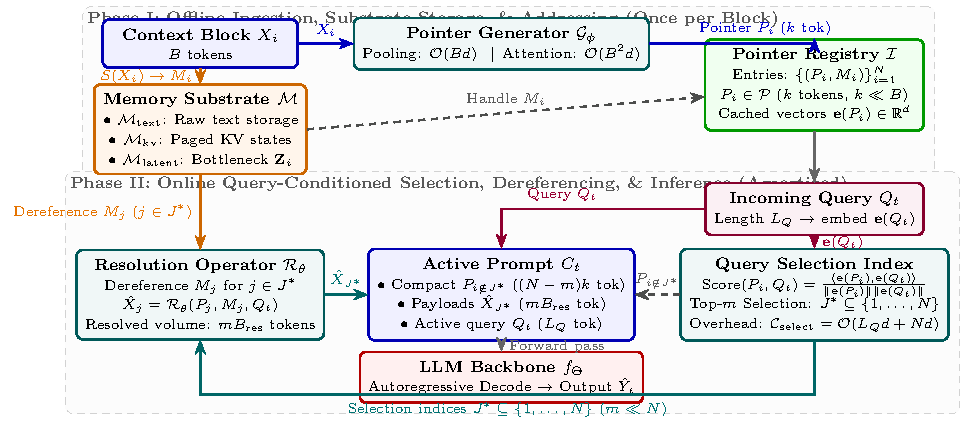
\includegraphics[width=0.66\textwidth]{figure_architecture.pdf}
\caption{The SemPointer architectural lifecycle and multi-tier memory substrate. (Top) Phase~I (Offline Ingestion and Addressing): Context block $X_i$ ($B$ tokens) is committed to substrate $\mathcal{M}$ ($\mathcal{M}_{\mathrm{text}}, \mathcal{M}_{\mathrm{kv}}, \mathcal{M}_{\mathrm{latent}}$) via $\mathcal{S}$, while generator $\mathcal{G}_\phi$ produces $k$-token pointer $P_i$, registered in index $\mathcal{I}$ with cached projection vector $\mathbf{e}(P_i) \in \mathbb{R}^d$. (Bottom) Phase~II (Online Query Selection and Resolution): Query $Q_t$ ($L_Q$ tokens) scores against $\mathcal{I}$ to select sparse subset $J^* \subseteq \{1,\dots,N\}$ ($m \ll N$). Resolution operator $\mathcal{R}_\theta$ dereferences active blocks $M_j$ into payloads $\hat{X}_j$, which combine with passive unselected pointers $P_{i \notin J^*}$ and query $Q_t$ into active prompt $C_t$ for autoregressive decode by LLM backbone $f_\Theta$.}
\label{fig:architecture}
\end{figure}

\subsection{Mathematical Model}
The model operates over five spaces, depicted in Fig.~\ref{fig:architecture} across its offline ingestion and online query lifecycles. Context Space $\mathcal{X}$ contains textual sequences $X \in \mathcal{V}^*$. Substrate Space $\mathcal{M}$ holds independent storage representations (raw text, KV tensors, or latent embeddings). Pointer Space $\mathcal{P}$ consists of sequences of $k$ discrete tokens or soft embeddings, with $k$ fixed and small ($k \in [1, 8]$). Query Space $\mathcal{Q}$ contains active prompts, and Output Space $\mathcal{Y}$ contains target generations.

\noindent\textbf{1) Encounter and Substrate Ingestion:}
When context item $X_i$ is encountered at time $t_i$, the storage operator $\mathcal{S}$ commits $X_i$ to substrate $\mathcal{M}$ while pointer generator $\mathcal{G}_{\phi}$ produces the compact semantic pointer:
\begin{equation}
M_i = \mathcal{S}(X_i), \quad P_i = \mathcal{G}_{\phi}(X_i) = (p_{i,1}, \dots, p_{i,k})
\end{equation}
The pair $(P_i, M_i)$ is registered in pointer index $\mathcal{I}_{t_i} = \mathcal{I}_{t_{i}-1} \cup \{(P_i, M_i)\}$.

\noindent\textbf{2) Query-Conditioned Selection:}
Upon arrival of query $Q_t$, registered pointers are scored via normalized inner product:
\begin{equation}\label{eq:scoring}
s_i = \operatorname{Score}(P_i, Q_t) = \frac{\langle \mathbf{e}(P_i), \mathbf{e}(Q_t) \rangle}{\|\mathbf{e}(P_i)\| \|\mathbf{e}(Q_t)\|}
\end{equation}
where, as executed, $\mathbf{e}(\cdot)$ is the frozen \texttt{sentence-transformers/all-MiniLM-L6-v2} mean-pooled block/query embedding (pointer ID strings excluded from scoring inputs). The system selects top-$m$ pointers $J^* = \operatorname{top-}m (\{s_i\}_{i=1}^N)$. Per-query selection work scales with the $N{\cdot}k{\cdot}d$ scoring tensor plus top-$m$ sort plus one query encode; no cross-query caching saving is claimed.

\noindent\textbf{3) Pointer Dereferencing and Resolution:}
For each selected index $j \in J^*$, executed resolution is verbatim dict lookup $\hat{X}_j = \mathcal{R}_{\theta}(P_j, M_j)$ returning stored $X_j$ with no $Q_t$-conditioning; joint composition $P_a \oplus P_b$ in \eqref{eq:composition} is specified-not-implemented. Resolved information $\hat{X}_{J^*}$ is injected into the generation prompt alongside unselected pointers:
\begin{equation}
\hat{Y}_t \sim f_{\Theta}\left(\cdot \mid [\{P_i\}_{i \notin J^*}, \hat{X}_{J^*}, Q_t]\right)
\end{equation}
Because unselected blocks remain represented by their compact pointers $P_i$ ($i \notin J^*$), active context consumes $L_{\mathrm{active}} = (N - m)k + \sum_{j \in J^*} |\hat{X}_j| + |Q_t| \le Nk + m B_{\mathrm{res}} + L_Q$ tokens, compared to $NB + L_Q$ in linear re-ingestion. $L_{\mathrm{active}}$ counts core pointer, resolved-block, and query tokens only, excluding instruction and framing tokens. Because all $N-m$ unselected pointers remain in the sequence, attention across the active prompt remains quadratic in $L_{\mathrm{active}}$; SemPointer reduces sequence length by replacing unselected blocks of size $B$ with pointers of size $k \ll B$, compressing the quadratic attention coefficient rather than altering the asymptotic polynomial degree.

\subsection{Concrete Instantiation: Generator and Resolver Mechanics}
Algorithm~\ref{alg:sempointer} formalizes the operational lifecycle implemented in our framework. To eliminate training artifacts and domain-specific bias, our primary realization employs a zero-shot, training-free pointer generator $\mathcal{G}_\phi$ and deterministic substrate resolvers $\mathcal{R}_\theta$:
\begin{itemize}\setlength{\itemsep}{0.5pt}\setlength{\parsep}{0pt}\setlength{\topsep}{1pt}
    \item \textbf{Training-Free Generator ($\mathcal{G}_\phi$):} In the reported runs, dense addressing projection $\mathbf{e}(P_i)$ is generated via the frozen public encoder \texttt{sentence-transformers/all-MiniLM-L6-v2} with mean pooling over per-block window embeddings (Section~\ref{sec:methods-selection}); discrete prompt handles are seeded random-projection buckets over the same embedding ($k$ tokens). Other generator realizations (attention-class readouts, TF-IDF handles, soft-prompt expansion) are specified as design alternatives in the cost model but were not executed. Because $\mathcal{G}_\phi$ operates entirely zero-shot over frozen pre-trained representations, parameter training requires zero optimization steps, zero fine-tuning data, and incurs zero unamortized training compute ($\mathcal{C}_{\mathrm{train}}=0$).
    \item \textbf{Deterministic Resolvers ($\mathcal{R}_\theta$):} For text substrate $\mathcal{M}_{\mathrm{text}}$, $\mathcal{R}_\theta$ performs exact in-memory index dereferencing returning the verbatim string $X_i$. For key-value cache $\mathcal{M}_{\mathrm{kv}}$, $\mathcal{R}_\theta$ performs physical memory block dereferencing, injecting cached KV tensors into attention tables ($\mathcal{C}_{\mathrm{res}} \approx 0$). Neither resolver requires learned parameters, guaranteeing exact resolution fidelity ($\epsilon=0$).
\end{itemize}

\begin{algorithm}[t]
\caption{Lifecycle of SemPointer Addressing and Resolution.}\label{alg:sempointer}
\begin{algorithmic}[1]
\footnotesize
\REQUIRE Stream $\mathcal{S}_{\text{stream}}$, Queries $\{Q_t\}$, Storage $\mathcal{S}$, Generator $\mathcal{G}_{\phi}$, Resolver $\mathcal{R}_{\theta}$, LLM $f_{\Theta}$
\STATE Initialize Pointer Registry $\mathcal{I} \leftarrow \emptyset$
\FORALL{context blocks $X_i \in \mathcal{S}_{\text{stream}}$}
    \STATE $M_i \leftarrow \mathcal{S}(X_i)$; \quad $P_i \leftarrow \mathcal{G}_{\phi}(X_i)$; \quad $\mathcal{I} \leftarrow \mathcal{I} \cup \{(P_i, M_i)\}$
\ENDFOR
\FORALL{queries $Q_t$}
    \STATE Score $s_i = \operatorname{Score}(P_i, Q_t)$ for $(P_i, M_i) \in \mathcal{I}$; \quad $J^* \leftarrow \operatorname{top-}m(\{s_i\}_{i=1}^N)$
    \STATE Active memory payload $\Omega_t \leftarrow \bigcup_{j \in J^*} \{\mathcal{R}_{\theta}(P_j, M_j)\}$
    \STATE Active prompt $C_t \leftarrow [\{P_i\}_{i \notin J^*}, \Omega_t, Q_t]$; \quad Emit $\hat{Y}_t \leftarrow f_{\Theta}(C_t)$
\ENDFOR
\end{algorithmic}
\end{algorithm}

\subsection{Upgraded Architecture: Patterns Absorbed from 2025--2026 Systems}
The lifecycle above is the executed baseline. This subsection specifies the upgraded design, drawn from recent systems. Everything here is specified-not-implemented unless stated; no pilot exercises it.

\noindent\textbf{Two-stage selection.} Recent KV-cache work splits retrieval into a cheap prefilter plus a precise rerank: RocketKV compresses in two stages \cite{behnam2025rocketkv}, and SnapKV first observes a voting window before keeping clustered keys \cite{li2024snapkv}. The upgraded selector mirrors this. Stage~1 scores all $N$ addresses by pointer-ID overlap $\hat{s}_i$ at $O(1)$ each, producing a shortlist $C$ with $|C| = c \ll N$. Stage~2 runs dense cosine only on $C$. Per-query selection drops from $O(N{\cdot}d)$ dense scoring to $O(N + c{\cdot}d)$. The executed system runs Stage~2 only, over all $N$.

\noindent\textbf{Adaptive per-block budgets.} Instead of fixed $k$, each block carries $k_i$ pointer tokens under a registry budget $\sum_i k_i \le K$. Salient blocks (high query-hit rate, high recency) earn longer addresses; cold blocks shrink to $k_i = 2$. Selection then maximizes expected utility per token, a knapsack allocation the fixed-$k$ runs do not attempt.

\noindent\textbf{Temporal versioning and edit operations.} Agent-memory systems converged on explicit mutation semantics: Mem0 routes every write through ADD, UPDATE, or DELETE operations \cite{chhikara2025mem0}, and Zep versions facts with valid-time intervals so history survives edits \cite{rasmussen2025zep}. The upgraded registry adopts four operations. REBIND$(P, M')$ atomically repoints a live handle at new content and bumps its version. FORGET$(P)$ writes a tombstone; dereferencing a tombstoned handle fails closed, never silently resurrects text. ALIAS$(P, Q)$ registers a second stable handle on one target with a reference count. DEREF$(P)$ resolves to the current target or raises the tombstone. None of these execute in the reported runs; the pilots mutate nothing.

\noindent\textbf{Query-aware scoring rule.} Quest scores each KV page against the live query vector and loads only Top-$K$ pages \cite{tang2024quest}. The upgraded selection rule has the same shape: score each address against $\mathbf{e}(Q_t)$, resolve the top $m$, page the rest out. Quest's bound is per-decoding-step over KV pages; ours is per-query over prompt-resident addresses, which leaves a persistent handle where Quest leaves none.

\noindent\textbf{What was deliberately not taken.} LLM-managed paging loops, in the MemGPT style \cite{packer2023memgpt}, trade determinism for autonomy; each eviction decision costs an LLM call and failures compound across turns, so orchestration stays outside the model here. Custom attention operators, in the Landmark style \cite{mohtashami2023landmark}, require retraining and break pretrained compatibility; addressing stays in token space for that reason. Full-KV retention with selective recompute, in the CacheBlend style \cite{yao2025cacheblend}, repairs cross-chunk attention at the price of keeping every chunk's KV resident; the text substrate sidesteps that cost by re-ingesting verbatim text only for resolved blocks.

\section{Memory Substrates and Physical Taxonomies}\label{sec:substrates}

{\small
Three realizations of $M_i$ trade off cost, capacity, and fidelity.

\noindent\textbf{A. Raw Text Substrate ($\mathcal{M}_{\text{text}}$):}
Holds $M_i = X_i$ in flat storage (RAM/disk); activation fetches $X_i$ into context. No encoding penalty or fidelity loss, but resolution pays I/O plus re-encoding.

\noindent\textbf{B. Key-Value Cache Substrate ($\mathcal{M}_{\text{kv}}$):}
Future work only: $M_i = (\mathbf{K}_i, \mathbf{V}_i) \in \mathbb{R}^{2 \times L_{\text{layers}} \times |X_i| \times d}$, precomputed in host or paged GPU memory \cite{kwon2023pagedattention}; resolution pages KV blocks in with $\mathcal{C}_{\mathrm{res}} \approx 0$ FLOPs. Capacity-bound: at fp16, a $B{=}512$ block at 70B scale ($n_{\mathrm{layers}}{=}80, n_{\mathrm{heads}}{=}64, d_{\mathrm{head}}{=}128$) occupies $\approx 1.34$\,GB, so $N \ge 10^3$ blocks need terabyte-scale storage; RoPE displacement $\Delta t$ can degrade relocated blocks.

\noindent\textbf{C. Latent Embedding Substrate ($\mathcal{M}_{\text{latent}}$, future work):}
$M_i = \mathbf{Z}_i \in \mathbb{R}^{m_z \times d}$ with $m_z \ll |X_i|$ from an autoencoder \cite{ge2024icae}, resolved by cross-attention unpooling over $\mathbf{Z}_i$ conditioned on $P_i, Q_t$; compact but lossy. No such module is trained and no reported run exercises it (all measurements use $\mathcal{M}_{\text{text}}$, Section~\ref{sec:methods-scope}).

\begin{table}[t]
\centering
\renewcommand{\arraystretch}{0.95}
\setlength{\tabcolsep}{3pt}
{\footnotesize
\begin{tabular}{@{}lp{3.2cm}p{3.2cm}p{3.5cm}@{}}
\toprule
\textbf{Property}
  & \textbf{$\mathcal{M}_{\text{text}}$ (Raw Text)}
  & \textbf{$\mathcal{M}_{\text{kv}}$ (KV Cache)}
  & \textbf{$\mathcal{M}_{\text{latent}}$ (Latent)} \\
\midrule
Storage
  & Flat text buffer (RAM/disk)
  & $(\mathbf{K}_i,\mathbf{V}_i)\!\in\!\mathbb{R}^{2\times L\times|X_i|\times d}$, precomputed
  & $\mathbf{Z}_i\!\in\!\mathbb{R}^{m_z\times d}$, $m_z\!\ll\!|X_i|$ \\
Resolution
  & Re-tokenize \& re-ingest $X_i$
  & Page KV blocks into attention tables
  & Cross-attention unpooling over $\mathbf{Z}_i$ \\
$\mathcal{C}_{\mathrm{res}}$
  & $\mathcal{O}(B_{\mathrm{res}}\,d^2)$ (re-encode)
  & $\approx 0$ FLOPs
  & $\mathcal{O}(m B_{\mathrm{res}} k d)$ \\
Fidelity
  & Lossless ($\varepsilon\approx 0$)
  & Lossless; RoPE displacement risk
  & Lossy ($\varepsilon>0$, bottleneck-dependent) \\
Bottleneck
  & I/O latency \& re-encoding cost
  & Memory capacity \& paging bandwidth
  & Reconstruction fidelity; hallucination risk \\
\bottomrule
\end{tabular}
}
\caption{The three SemPointer memory substrates compared: $\mathcal{M}_{\text{text}}$ lossless with re-encoding cost; $\mathcal{M}_{\text{kv}}$ zero-FLOP resolution but capacity-bound; $\mathcal{M}_{\text{latent}}$ compact but lossy.}
\label{tab:substrates}
\end{table}

\enlargethispage{2\baselineskip}
\section{Theoretical Complexity and Cost Modeling}\label{sec:complexity}

\subsection{Modeling Assumptions}
We compare indirection against linear re-ingestion under five assumptions:
\begin{itemize}\setlength{\itemsep}{0.5pt}\setlength{\parsep}{0pt}\setlength{\topsep}{1pt}
    \item[\textbf{A1.}] \textbf{Uniform Block Partitioning:} Context splits into $N$ blocks of length $B$ ($L_H = N \cdot B$).
    \item[\textbf{A2.}] \textbf{Sparse Access Frequency:} Across $K$ queries (each length $L_Q$), each query accesses on average $m \ll N$ units (deterministic expectation).
    \item[\textbf{A3.}] \textbf{Compact Pointer Invariant:} Each pointer is $k$ tokens with $k \ll B$ (Axiom~\ref{ax:compactness}).
    \item[\textbf{A4.}] \textbf{Upfront Amortization:} Initial encoding and pointer generation ($\mathcal{C}_{\text{init}}$) run once and amortize over later queries.
    \item[\textbf{A5.}] \textbf{Cached Addressing Embeddings:} Projections $\mathbf{e}(P_i)$ are cached at registration; scoring needs one $\mathbf{e}(Q_t)$ plus $N$ inner products, so $\mathcal{C}_{\mathrm{select}}=\mathcal{O}(L_Q d + Nd)$ per \eqref{eq:scoring}, as required by Axioms~\ref{ax:stability}--\ref{ax:reusability}. Fine-tuning invalidates the cache.
\end{itemize}

\subsection{Resolution Cost by Substrate}
Resolution cost $\mathcal{C}_{\mathrm{res}}(m,B_{\mathrm{res}},Q_t)$ follows Section~\ref{sec:substrates}: $\mathcal{M}_{\mathrm{text}}$ re-encodes ($\mathcal{C}_{\mathrm{res}} = m(2dB_{\mathrm{res}}^2 + 4d^2B_{\mathrm{res}})$); $\mathcal{M}_{\mathrm{kv}}$ reuses paged KV ($\mathcal{C}_{\mathrm{res}} \approx 0$ recompute FLOPs, excluding I/O and paged-attention paging latency/bandwidth); $\mathcal{M}_{\mathrm{latent}}$ costs $\mathcal{O}(m B_{\mathrm{res}} k d)$.

\subsection{Asymptotic FLOPs Analysis}
Consider hidden dimension $d$.\footnote{We suppress layer-dependent constant factors ($n_{\text{layers}}$, $n_{\text{heads}}$); see Section~\ref{sec:background} for the expanded KV-state expression.} We compare cost across $K$ queries.

\noindent\textbf{1) Linear Re-Ingestion Paradigm:}
Each query re-attends to full history $L_H$:
\begin{align}
    \mathcal{C}_{\text{linear}} &= K \left[ 2 d (NB + L_Q)^2 + 4 d^2 (NB + L_Q) \right] \nonumber \\
&\approx 2 K d (NB + L_Q)^2
\end{align}

\noindent\textbf{2) SemPointer Indirection Paradigm:}
\begin{enumerate}\setlength{\itemsep}{1pt}\setlength{\parsep}{0pt}\setlength{\topsep}{1.5pt}
    \item \textbf{One-Time Generation and Storage:}
    \begin{equation}
    \mathcal{C}_{\text{init}} = N \cdot \left[ 2 d B^2 + 4 d^2 B + \mathcal{C}_{\text{gen}}(B, k) \right]
    \end{equation}
    Note $4d^2B$ dominates $2dB^2$ when $B < 2d$ (typical: $B \le 10^3$, $d \geq 4096$). Pooling-class $\mathcal{C}_{\text{gen}}$ costs $\mathcal{O}(Bd)$; attention readouts (Corollary~1) cost $\mathcal{C}_{\text{gen}} = c_g(2dB^2 + 4d^2 B)$, $c_g = \Theta(1)$. Our pooling generator is training-free ($\mathcal{C}_{\mathrm{train}}=0$). Proposition~\ref{prop:single_query} covers $\mathcal{C}_{\mathrm{gen}} \ge \Omega(Bd)$; Corollary~1 covers attention-class generators.
    \item \textbf{Per-Query Pointer Selection:} $\mathcal{C}_{\mathrm{select}} = \mathcal{O}(L_Q d + Nd)$ (Eq.~\eqref{eq:scoring}, A5).
    \item \textbf{Per-Query Resolution and Inference:} Active prompt holds $N-m$ pointers, $m$ resolved blocks ($B_{\text{res}} \le B$), and $Q_t$:
    \begin{equation}\label{eq:active_seq}
    L_{\mathrm{active}} = (N-m)k + m B_{\mathrm{res}} + L_Q \le Nk + m B_{\mathrm{res}} + L_Q
    \end{equation}
    Per-query cost:
    \begin{equation}
    \mathcal{C}_{\text{query}} = 2 d\, L_{\mathrm{active}}^2 + 4 d^2 L_{\mathrm{active}} + \mathcal{C}_{\text{res}}(m, B_{\text{res}}, Q)
    \end{equation}
\end{enumerate}
Summing over $K$ queries:
\begin{align}
\mathcal{C}_{\text{SemPointer}} &= \mathcal{C}_{\mathrm{init}} + K[\mathcal{C}_{\mathrm{select}} + \mathcal{C}_{\mathrm{query}}] \nonumber \\
&= N(2dB^2 + 4d^2B + \mathcal{C}_{\mathrm{gen}}) \nonumber \\
&\quad + K\big[2dL_{\mathrm{active}}^2 + 4d^2 L_{\mathrm{active}} + \mathcal{C}_{\mathrm{res}} + \mathcal{C}_{\mathrm{select}}\big]
\end{align}

\enlargethispage{2\baselineskip}
\subsection{The Indirection Crossover Threshold}

\begin{proposition}[Crossover Threshold]\label{prop:crossover}
Under A1--A5, indirection
yields lower cumulative FLOPs than linear re-ingestion iff
(i) $\Delta\mathcal{C}_{\mathrm{step}} > 0$ --- up to overheads, equivalently
 $N(B-k) > mB_{\text{res}}$ --- and (ii) $K > K^\ast =
\mathcal{C}_{\mathrm{init}}/\Delta\mathcal{C}_{\mathrm{step}}$:
\begin{equation}
K^* = \frac{\mathcal{C}_{\mathrm{init}}}{\Delta\mathcal{C}_{\mathrm{step}}}
\end{equation}
where the per-query marginal savings $\Delta\mathcal{C}_{\mathrm{step}}$ is given by:
\begin{align}\label{eq:delta_step}
\Delta\mathcal{C}_{\mathrm{step}} &= \big[N(B-k) - m(B_{\mathrm{res}}{-}k)\big] \nonumber \\
&\quad \cdot \Big[2d\big(N(B{+}k) + m(B_{\mathrm{res}}{-}k) + 2L_Q\big) + 4d^2\Big] \nonumber \\
&\quad - \mathcal{C}_{\mathrm{select}} - \mathcal{C}_{\mathrm{res}}
\end{align}
If $m(B_{\mathrm{res}}{-}k) \geq N(B-k)$,
indirection is dominated for every $K$. Both $K^\ast$ and $\Delta\mathcal{C}_{\mathrm{step}}$ are analytic: no $K$-sweep is measured (operating points overlaid in Section~\ref{sec:regime-map}).
\end{proposition}

\textit{Derivation.} Difference-of-squares on $(L_H{+}L_Q)^2 - L_{\mathrm{active}}^2$ plus the $4d^2$ projection difference yields \eqref{eq:delta_step}: (tokens avoided) $\times$ (per-token coefficient) minus addressing and resolution overheads. Latency is logged (\texttt{GenResult.latency\_ms}, TTFT tap in \texttt{experiments/engine/llm.py}) and reported in Table~\ref{tab:N3-efficiency}, without a FLOPs-crossover fit.

\begin{proposition}[Single-Query Viability]\label{prop:single_query}
Under A1--A5 with the $\mathcal{M}_{\text{kv}}$ substrate ($\mathcal{C}_{\mathrm{res}}\approx 0$), $L_Q \ll NB$, and sparse access ($mB_{\text{res}} \ll NB$), $K^* < 1$ reduces to $N > 1 + \mathcal{O}(k/B + dk/B^2)$. Under pooling-class generation, $N \ge 2$ satisfies it. At $N=1$, indirection does not amortize on the first query ($K^* \approx 1.015 > 1$ for $d=4096, B=512, k=8, \mathcal{C}_{\mathrm{gen}}=Bd$), whereas at $N=2$ ($K^* \approx 0.958 < 1$) it does. This illustration is analytic (no $N{=}1$-vs-$2$ run exists). Quoted $K^*$ values are boundary-case illustrations at helper defaults $m{=}0$, $L_Q{=}0$, $\mathcal{M}_{\mathrm{kv}}$ (optimistic: zero payload/resolution cost; $m{\ge}1$ raises $K^*$). The $d{=}4096$ illustrations do not transfer to the Qwen2.5-3B reader. Under $\mathcal{M}_{\text{text}}$, where $\mathcal{C}_{\mathrm{res}}$ reinstates quadratic cost per query, $K^*$ exceeds 1 and multi-query amortization governs.
\end{proposition}

\vspace{0.3em}
\noindent\textbf{Corollary 1 (Attention-Class Pointer Generators).} Proposition~2 assumes pooling-class $\mathcal{C}_{\mathrm{gen}}=\mathcal{O}(Bd)$ (e.g., readout pooling over precomputed token embeddings). If $\mathcal{G}_\phi$ is attention-based, $\mathcal{C}_{\mathrm{gen}} = c_g(2dB^2 + 4d^2B)$, $c_g=\Theta(1)$, and viability reduces to $N > (1+c_g) + (2d/B)\,c_g$. For $c_g=1$: $N \gtrsim 2 + 2d/B$ (e.g., $N \gtrsim 18$ at $d{=}4096$, $B{=}512$; $N \gtrsim 6$ at $B{=}2048$). Below the threshold, Proposition~1 multi-query amortization applies. Analytic only: no attention-class generator is built or timed in the present runs.

\vspace{0.5em}
\noindent\textbf{Remark 1 (Scope of Comparison).} $\mathcal{C}_{\mathrm{linear}}$ models the no-cache regime: stateless inference, API access, cache eviction
between sessions, or contexts exceeding cache capacity. Against a
persistent KV cache with host offload~\cite{kwon2023pagedattention}, per-query recompute FLOPs
approach zero and the binding resource is memory capacity and paging
bandwidth; there SemPointer retains only $Nk$ pointer tokens in fast memory.

\begin{table}[t]
\caption{Architectural Comparison of Context-Management and Memory Approaches. Entries characterize each system at the level of its published description; see Section~VIII-B for a comparison of composable addressing (Axiom~7) against standard RAG concatenation.}\label{tab:feature_matrix}
\centering
\renewcommand{\arraystretch}{0.88}
\resizebox{\textwidth}{!}{%
\begin{tabular}{@{}lccccccc@{}}
\toprule
\textbf{Framework} & \textbf{Primary Representation} & \textbf{Representation Type} & \textbf{Decoupled Substrate?} & \textbf{Explicit Address?} & \textbf{Selective Access?} & \textbf{Composable Addressing?} & \textbf{Multi-Turn Reusability?} \\ \midrule
Gist Tokens \cite{mu2023gist} & Soft Tokens & Continuous & No & No & No & No & Yes \\
AutoCompressors \cite{chevalier2023autocompressors} & Summary Vectors & Continuous & No & No & No & No & Yes \\
ICAE \cite{ge2024icae} & Memory Slots & Continuous & No & No & No & No & Yes \\
500xCompressor \cite{li2025500xcompressor} & Special Tokens & Discrete/Latent & No & No & No & No & No \\
SAC \cite{liu2025sac} & Anchor Tokens & Token KV & No & No & No & No & No \\
CCM \cite{kim2024ccm} & Compressed KV & KV Tensors & Yes (KV) & No & No & No & Yes \\
LLMLingua-2 \cite{pan2024llmlingua2} & Pruned Text & Discrete Text & No & No & No & No & No \\
xRAG \cite{cheng2024xrag} & Document Embedding & Continuous & Yes (Ext DB) & Partial (dense; same family) & Yes (Retrieval) & No & Yes \\
MemGPT \cite{packer2023memgpt} & Page ID / Chunks & Positional/Text & Yes (Archival) & Yes (page-ID; positional) & Yes (Tool-Call) & No & Yes \\
Landmark Attention \cite{mohtashami2023landmark} & Landmark Tokens & Token Markers & No & No (intra-pass routing) & Yes (Blocks) & No & No \\
\textbf{SemPointer (Proposed)} & \textbf{Semantic Pointer} & \textbf{Token Seq. / Latent} & \textbf{Yes (Multi-tier)} & \textbf{Yes (Semantic)} & \textbf{Yes (Query-Cond.)} & \textbf{No (specified, untested)} & \textbf{Yes} \\ \bottomrule
\end{tabular}%
}
\end{table}



\section{Theoretical Vulnerabilities and Failure Modes}

\noindent\textbf{A. Address Collision via Generalized Birthday Bounds:}
\begin{proposition}[Combinatorial Address Collision Bound]\label{prop:collision}
Let pointer space $\mathcal{P}$ consist of sequences of length $k$ over discrete vocabulary $\mathcal{V}_p$ of size $V = |\mathcal{V}_p|$. Under independent, uniformly distributed pointer generation, the probability that any two of $N$ registered memory items share an identical address is bounded by $P_{\text{collision}} \approx 1 - \exp\left(-\frac{N(N-1)}{2 V^k}\right)$.
\end{proposition}

\textit{Proof Sketch.} Birthday bound over $|\mathcal{P}|=V^k$ under uniform assignment; equal-width binning is non-uniform (\texttt{pointer\_generator.py}); no collision rate is logged. Hence the uniform-distribution bound contradicts the actual generator and serves as an analytic illustration only, not a guarantee for the reported runs.

\begin{proposition}[Combinatorial Address Space Capacity]\label{prop:capacity}
Under the uniform birthday-bound model, to maintain collision probability below threshold $\delta$ across a memory registry of $N$ items, the minimum discrete pointer length $k$ must satisfy $k \ge \left\lceil \frac{\ln(N^2) - \ln(2 \delta)}{\ln V} \right\rceil$.
For illustration, with $N = 10^5$, $V = 32{,}000$, and $\delta = 10^{-4}$: $k \ge \lceil \frac{23.02 + 8.51}{10.37} \rceil = 4$.
This calculation concerns combinatorial capacity; Proposition~4's lower bound ($k \ge 4$ under $N=10^5$, $V=32{,}000$, $\delta=10^{-4}$) and Axiom~2's compactness jointly restrict viable pointer length to $k \in [4, 8]$. Analytic illustration only: all reported runs use $k=8$, which satisfies the bound without testing it (\texttt{config\_table.json}). Tested registries average $N{\approx}25$--$28$ blocks per example (Section~\ref{sec:methods}), so the $N{=}10^5$ calculation is untested analytic extrapolation, not a validated scale claim.
\end{proposition}

\noindent\textbf{B. Semantic Drift Across Extended Horizons (assumption; future measurement):}
Phenomenological ansatz (not from RoPE geometry): attention may decay with displacement $\Delta t = t_{\text{curr}} - t_{\text{gen}}$ as: $\mathbb{E}[\alpha(Q_t, P_i)] \propto \exp(-\lambda |t - t_i|)$, where $\lambda > 0$ is unspecified. Unmeasured; future work.

\noindent\textbf{C. Resolution Divergence and Hallucination:}
On lossy $\mathcal{M}_{\text{latent}}$, reconstructions may deviate: $\mathcal{D}_{\text{KL}}(p(X_i) \parallel p(\hat{X}_i \mid P_i, M_i)) > 0$. Beyond tolerance this hallucinates, so precision-critical tasks assume $\mathcal{M}_{\text{text}}$ or $\mathcal{M}_{\text{kv}}$; no $\mathcal{M}_{\text{latent}}$ run exists (future work, Section~\ref{sec:substrates}).

\noindent\textbf{D. Prompt Injection via PTR Strings:}
Untrusted block text resolved via $\mathcal{M}_{\text{text}}$ renders verbatim into the active prompt, so a malicious instruction in a selected block could steer $f_\Theta$; pointer identifier strings are likewise prompt-resident. No adversarial or injection test was run, so this is an untested threat model, not a measured vulnerability.

\begin{figure}[t]
\centering
\includegraphics[width=0.70\textwidth]{figures/N1_pareto.pdf}
\caption{Lead result: measured accuracy versus measured active tokens (Pareto plane), one panel per suite, with 95\% CIs. SemPointer sits an order of magnitude left of full context on tokens at lower accuracy, and ties dense RAG at higher token cost. KV-compress pilot omitted (n=10).}
\label{fig:N1-pareto}
\end{figure}

\section{Critical Boundary Analysis and Literature Comparison}

\noindent\textbf{A. Disambiguation from Landmark Attention:}
Landmark Attention \cite{mohtashami2023landmark} routes attention across blocks via tokens. Three differences separate it from SemPointer: (1)~\emph{Routing vs.\ persistent indirection:} Landmark gates attention within a continuous sequence; SemPointer dereferences an independent substrate across queries via an address registry. (2)~\emph{Transient marker vs.\ address handle:} landmark tokens are routing gates; SemPointers are persistent handles (composition specified, untested). (3)~\emph{Eviction:} Landmark keeps full context or KV states active; SemPointer offloads substrate to secondary storage, retaining only $k$ tokens per block.

\noindent\textbf{B. Disambiguation from Retrieval-Augmented Generation:}
RAG \cite{lewis2020rag, cheng2024xrag} and SemPointer both select over external stores but differ in addressing. Standard RAG appends retrieved blocks to context, leaving relational binding to downstream self-attention. SemPointer defines composable references ($P_a \oplus P_b$) registered and dereferenced jointly (Axiom~\ref{ax:compositionality}, \eqref{eq:composition}). Joint resolution is specified but untested here: the multi-hop pilot (Table~\ref{tab:N6-pilot}) favors dense top-$1$ over index-routed resolution. For two-hop query (\textit{``What did the vendor in turn 12 quote in turn 40's email?''}), RAG concatenates both blocks, whereas SemPointer forms joint address $(P_{12} \oplus P_{40})$ resolved once against $\{M_{12}, M_{40}\}$ conditioned on $Q_t$.

\noindent\textbf{C. Disambiguation from Operating-System-Style Memory (MemGPT):}
MemGPT \cite{packer2023memgpt} moves text blocks between active context and archival storage via function calls and parser interrupts. Three distinctions separate SemPointer: (1)~\emph{Addressing:} MemGPT uses integer page IDs or metadata via system instructions and tool calls; SemPointer uses token-level addresses from $\mathcal{G}_\phi$ in sequence space. (2)~\emph{Integration:} evicted MemGPT pages leave no active trace and need explicit tool invocation; unselected SemPointer blocks retain $k$-token pointers ($P_{i \notin J^*}$) in attention, preserving global presence while payloads stay offloaded. (3)~\emph{Complexity:} MemGPT is an empirical systems framework; SemPointer gives closed-form derivations (Propositions~1--2) for when indirection amortizes against re-ingestion.

\enlargethispage{2\baselineskip}
\noindent\textbf{D. Feature-Level Comparison with Related Approaches:}
Table~\ref{tab:feature_matrix} contrasts SemPointer with representative compression and memory architectures across seven dimensions.
\textbf{Explicit Address and Decoupled Substrate:} Gist Tokens \cite[§2]{mu2023gist}, AutoCompressors \cite[§3.1]{chevalier2023autocompressors}, and ICAE \cite[§2]{ge2024icae} are address-less prefixes with no substrate. 500xCompressor \cite[§3]{li2025500xcompressor} collapses context into one token. CCM \cite[§3.2]{kim2024ccm} offloads merged KV (\emph{Yes (KV)}) with no explicit address (\emph{No}). xRAG \cite[§2.2]{cheng2024xrag} retrieves by dense-vector selection in the same family as ours (\emph{Partial}, \emph{Yes (Ext DB)}). MemGPT \cite{packer2023memgpt} page-IDs are explicit addresses, so marked \emph{Yes}; the distinction is address-type only (positional page-ID vs.\ semantic) with \emph{Yes (Archival)} substrate. Landmark \cite[§3]{mohtashami2023landmark} tokens route blocks intra-pass within one pass, hence \emph{No} explicit cross-query address.
\textbf{Composition (Axiom~7):} AutoCompressor vectors \cite[§3.1]{chevalier2023autocompressors} lack an algebra for non-adjacent references (\emph{No}). Gist Tokens \cite{mu2023gist} and ICAE \cite{ge2024icae} leave binding to attention over summaries. Landmark \cite[§3]{mohtashami2023landmark} routes within-sequence with no cross-turn handles (\emph{No}). SemPointer specifies composition ($P_a \oplus P_b$, \eqref{eq:composition}) but it is untested here, hence marked \emph{No (specified, untested)}.
\noindent\textbf{E. Query-Aware Sparsity and KV-Reuse Systems:} Three systems implement the dense-selection half of SemPointer's pipeline and bound its novelty. InfLLM \cite{xiao2024infllm} pairs sliding-window attention with block-level KV memory selected by attention scores, scaling to 1M tokens with no in-prompt handle. RetrievalAttention \cite{liu2025retrievalattention} offloads KV to CPU behind ANN indexes scanning 1--3\% of keys per step; addresses are transient hits, not authored tokens. Quest \cite{tang2024quest} loads Top-$K$ KV pages per query via attention bounds, leaving no residual handle. CacheBlend \cite{yao2025cacheblend} reuses precomputed KV of non-prefix chunks with selective recompute, keyed by chunk hash without query-conditioned selection. PromptCache \cite{gim2024promptcache} stitches position-correct cached KV modules across requests. Memorizing Transformers \cite{wu2022memorizing} bury kNN reads inside one attention layer with no textual address. Infini-attention \cite{munkhdalai2024infiniattention} folds past states into a fixed-size compressive matrix per attention block, retrieved by linear-attention lookup with a gate mixing long-term and local outputs. A second family pairs retrieval with compressed or embedded context and amortized or offline encoding across queries \cite{xu2024recomp, rau2025cocom, tan2024lloco, gao2025uniicl, tack2024mac}, while token-level reuse across requests targets decode acceleration \cite{luo2025recycling}. Against all six, SemPointer's defensible residual is narrow: prompt-resident textual pointers, verbatim-text (not KV) resolution, and specified-but-untested composition.

\section{Empirical Methods}\label{sec:experiments}\label{sec:methods}
% Condensed methods summary (~40 lines). Full detail moved verbatim to the
% supplementary file supplement_methods.tex (identical to sections/_methods.tex,
% retained in repo). All configuration facts are preserved below.
\subsection{System under test}\label{sec:methods-selection}
Context is chunked into blocks of at most $B=512$ tokens (reader tokenizer;
a trailing fragment shorter than $B/8$ merges into the previous block). Each block
carries one $k=8$ pointer; all final runs resolve $m=1$ block per query
(RAG baselines likewise retrieve $m=1$). Resolution uses $\mathcal{M}_{\mathrm{text}}$:
the selected block's verbatim text enters the prompt. Selection is dense cosine
similarity between mean-pooled query and per-block pointer embeddings from the
frozen public \texttt{sentence-transformers/all-MiniLM-L6-v2} encoder; blocks past
the encoder's maximum length are embedded whole via windowed mean-pooling
(\texttt{embed\_long}), never truncated. Pointer identifier strings
(\texttt{[PTR\_id: ...]}) are prompt-resident for unselected blocks only, carry
no key--value state, and do not affect selection; dense RAG sees identical
representations. KV ($\mathcal{M}_{\mathrm{kv}}$) and latent
($\mathcal{M}_{\mathrm{latent}}$) substrates are future work only\label{sec:methods-scope}: the KV-compress
pilot (Table~\ref{tab:N4-kv-pilot}) runs KVPress methods as black-box baselines at
$n=10$, not a SemPointer KV substrate. Four further implemented baselines (agentic
pointer routing, iterative RAG, hybrid fusion, session summaries) were not in the
final runs and carry no numbers here.
\subsection{Reader, suites, and metric adaptations}
All suites run on one reader (\texttt{Qwen/Qwen2.5-3B-Instruct}, NF4, greedy
decoding, seed~42) on a single 8\,GB GPU with CPU-only embedding fallback.
RULER ($n=180$ per system) re-implements the official generators and applies the
official per-sample containment rule ($1.0$ if the reference string appears, else
$0.0$). LongBench ($n=1150$; $1136$ scored for full context after 14 narrativeqa
OOMs, see \S\ref{sec:results-oom}) spans six tasks (hotpotqa \cite{yang2018hotpotqa}, 2wikimqa, musique \cite{trivedi2022musique},
multifieldqa\_en, narrativeqa \cite{kovcisky2018narrativeqa}, qasper) on official data, scored by verbatim
official normalization plus Counter-based token F1 maximized over ground truths.
LoCoMo ($n=199$ per system, ten official conversations) uses a stated token-F1
adaptation for \textit{all} categories---the official GPT-4 judge plus
Porter-stemmed F1 is unavailable---so no LoCoMo number here is comparable to
published LoCoMo results.
\subsection{Statistics and configuration ledger}
Comparisons use example-identifier-matched rows only (exact McNemar for binary
containment, Wilcoxon signed-rank for F1; paired bootstrap 95\% CIs with 10\,000
resamples at seed~42; Bonferroni $\alpha=0.05/13\approx 0.0038$). True mean tokens
per block are $506.6$/$504.2$/$510.2$/$487.9$ (RULER/LongBench/LoCoMo/KV pilot),
so $\kappa=k/B_{\mathrm{true}}\approx 0.016$ at $k=8$; mean blocks per example are
$24.75$/$26.67$/$28.0$/$7.5$. Recomputed score means match \texttt{metrics.json}
on every suite. Full protocols, code paths, and deviations are in the supplement.

\section{Results}\label{sec:results-measured}
{\small\input{tables/LNCS_N1_main_results}}
\input{tables/LNCS_N2_ruler_pertask}
% PAPER-A fragment: Results section. Owned by PAPER-A; do not edit from orchestrator wiring.
% Sources: stats.json (deltas/CIs/p-values/Bonferroni), error_breakdown.json
% (taxonomy), config_table.json, tables N1-N5. Tags: [ESTABLISHED] = measured;
% [REASONED] = direct inference, flagged. Losses are reported before any savings.
\label{sec:results}

\subsection{Suite summary: accuracy losses first}
\label{sec:results-summary}

Table~\ref{tab:N1-main} gives suite means with bootstrap 95\% CIs; paired
deltas, tests, and the Bonferroni family ($13$ tests, adjusted
$\alpha \approx 0.0038$) come from \texttt{stats.json}. Three of the 13
paired tests survive correction: RULER SemPointer-vs-full, RULER
SemPointer-vs-BM25, and LongBench SemPointer-vs-full [ESTABLISHED].

On RULER containment ($n=180$ matched pairs), SemPointer scores $0.3300$
against $0.7000$ for full context: paired delta $-0.37$,
95\% CI $[-0.44,-0.30]$, McNemar discordant $b=1$, $c=61$,
$p \approx 6.7\times10^{-14}$, surviving Bonferroni [ESTABLISHED]. Against
BM25 ($0.5778$) the delta is $-0.248$, CI $[-0.314,-0.183]$,
$p \approx 2.3\times10^{-10}$, likewise surviving [ESTABLISHED]. Against
dense RAG ($0.3289$), the pointer layer contributes essentially nothing: the
delta is $+0.0011$, CI $[-0.003,+0.006]$, with zero McNemar discordant pairs
($b=c=0$, $p=1.0$; Wilcoxon $p=0.65$) [ESTABLISHED]. The RAG and SemPointer
rows are near-identical across the whole taxonomy
(Table~\ref{tab:N5-taxonomy}: both hit~57, miss~123, retrieval-miss~51)
[ESTABLISHED].

On LongBench F1, SemPointer ($0.0773$, $n=1150$) trails full context
($0.1112$, $n=1136$ scored) by a paired delta of $-0.033$, CI
$[-0.040,-0.027]$ over $n=1136$ matched pairs, Wilcoxon
$p \approx 1.6\times10^{-31}$, surviving Bonferroni [ESTABLISHED].
SemPointer-vs-RAG is $-0.0009$, CI $[-0.0047,+0.0028]$, $p=0.32$, and
SemPointer-vs-BM25 is $-0.0040$, CI $[-0.010,+0.002]$, $p=0.156$: neither is
significant [ESTABLISHED]. Figure~\ref{fig:N1-pareto} places these
accuracy--cost trade-offs on one plane.

On LoCoMo with the token-F1 adaptation ($n=199$ matched pairs), SemPointer
($0.0518$) trails full context ($0.0642$) by $-0.012$, CI
$[-0.022,-0.003]$, Wilcoxon $p=0.028$ --- nominally positive but
\textit{not} significant after Bonferroni, so no difference is claimed
[ESTABLISHED]. SemPointer-vs-RAG ($+0.0017$, CI $[-0.005,+0.008]$,
$p=0.69$) and SemPointer-vs-BM25 ($-0.011$, CI $[-0.022,+0.001]$,
$p=0.037$) are likewise not significant after correction [ESTABLISHED].
No superiority over BM25 or full context is claimed on any suite
[REASONED].

\subsection{RULER per-task: easy parity, hard collapse}
\label{sec:results-ruler}

Table~\ref{tab:N2-ruler-pertask} and Figure~\ref{fig:N2-ruler} break RULER
into per-task cells of $n=30$. On the easiest needle task,
\texttt{niah\_single\_1}, SemPointer matches full context exactly
($0.9667 = 0.9667$) [ESTABLISHED]. Difficulty then separates the systems:
\texttt{niah\_single\_2} gives $0.2000$ against full context's $1.0000$,
\texttt{niah\_single\_3} gives $0.2667$ against $0.7000$, and
\texttt{multikey\_1} gives $0.4667$ against $0.9333$ [ESTABLISHED]. Variable
tracking (\texttt{vt}) and common-word extraction (\texttt{cwe}) are
collapses for every sparse system: SemPointer scores $0.0733$ on vt against
$0.5933$ for full context, while cwe sits at the floor ($0.0067$) for all
four systems including full context, a task-level bound rather than a
retrieval effect [ESTABLISHED]. BM25 exceeds SemPointer on the harder NIAH
cells ($0.8000$ and $0.6667$ on \texttt{single\_2}/\texttt{single\_3}),
consistent with lexical needles that survive sparse selection poorly under
dense cosine at $m=1$ [REASONED].

\subsection{Efficiency: large token and latency reductions at lower accuracy}
\label{sec:results-efficiency}

Table~\ref{tab:N3-efficiency} and Figure~\ref{fig:N3-efficiency} report
measured active tokens, end-to-end latency, and peak VRAM with sparse/full
ratios. SemPointer uses roughly one-tenth the active context of full
ingestion: $1270.3$ vs $13089.2$ tokens on RULER (ratio $0.097$),
$963.5$ vs $13066.1$ on LongBench ($0.074$), and $987.3$ vs $14525.1$ on
LoCoMo ($0.068$) --- about $10$--$15\times$ fewer tokens [ESTABLISHED].
Latency falls with prompt length: $894.5$ vs $7256.9$~ms on RULER
($0.123$, about $8\times$), $1527.2$ vs $8084.5$~ms on LongBench ($0.189$,
about $5\times$), and $1308.8$ vs $5326.2$~ms on LoCoMo ($0.246$, about
$4\times$) --- $5$--$8\times$ faster end to end on RULER and LongBench
[ESTABLISHED]. Peak VRAM drops from $3463.0$ to $2331.2$~MB on RULER
($0.673$), $2994.4$ to $2300.5$~MB on LongBench ($0.768$), and $3825.1$ to
$2302.6$~MB on LoCoMo ($0.602$) [ESTABLISHED]. These savings accompany the
accuracy losses of \S\ref{sec:results-summary}; they do not offset them, and
the paper makes no net-benefit claim [REASONED]. The pointer layer itself is
a small net cost over plain RAG: SemPointer feeds $+363$ more active tokens
per request than RAG on RULER ($1270.3$ vs $907.2$), about $+395$ on
LongBench and $+416$ on LoCoMo, for a measured RULER delta of $+0.001$
[ESTABLISHED].

\subsection{KV-compress pilot: no claims at \texorpdfstring{$n=10$}{n=10}}
\label{sec:results-kv}

Table~\ref{tab:N4-kv-pilot} reports the kv-compress pilot at $n=10$ with wide
CIs shown as-is. SemPointer scores $0.8000$ (CI $[0.60,1.00]$) against
$1.0000$ for full context (delta $-0.2$, CI $[-0.5,0.0]$, McNemar
$p=0.48$); against KVPress SnapKV~0.3 ($0.5000$) the delta is $+0.3$, CI
$[-0.1,+0.7]$, $p=0.37$; against ToVA~0.3 ($0.8000$) it is $0.0$, CI
$[-0.3,+0.3]$; against KNorm~0.3 ($0.4000$) it is $+0.4$, CI
$[+0.1,+0.7]$, McNemar $p=0.13$ [ESTABLISHED]. None of the four pilot tests
survives Bonferroni, and the pilot note in \texttt{stats.json} states that
no significance is claimed [ESTABLISHED]. The numbers are reported for
completeness only [REASONED].

\subsection{Failure taxonomy}
\label{sec:results-taxonomy}

Table~\ref{tab:N5-taxonomy} classifies every scored miss from
\texttt{error\_breakdown.json} (miss := score $< 1.0$ containment or
$< 0.5$ F1; retrieval-miss := miss with no selected block overlapping gold).
On RULER, SemPointer's 123 misses split into 51 retrieval-misses and 66
block-hit-wrong cases (gold block selected, answer still wrong), with 6
gold-not-localizable rows where the gold answer cannot be localized to any
chunk under the production chunking rule [ESTABLISHED]. The identical split
for dense RAG (51/66/6) confirms the selection stage, not the pointer
encoding, as the binding constraint [REASONED]. On LongBench the dominant
categories are retrieval-miss (465) and block-hit-wrong (253), but 409 of
1150 rows are gold-not-localizable: over a third of the suite cannot reward
any block selection under 512-token chunking, which compresses every
system's headroom [ESTABLISHED]. On LoCoMo, 157 of 199 rows are
gold-not-localizable for SemPointer (157 for full context as well), with
only 28 retrieval-misses and 14 block-hit-wrong; hit counts are 0 of 199
[ESTABLISHED]. Two structural failure modes recur across suites
[REASONED]: boundary-split needles, where a gold span straddles a 512-token
chunk edge so no single block contains it; and multihop splits, where the
two (hotpotqa/2wikimqa) or two-to-four (musique) supporting facts land in
different blocks while $m=1$ resolves exactly one. Per-task tables serve as
the hop breakdown because official hop-count labels are absent from the
items (\texttt{error\_breakdown.json}: design mapping hotpotqa/2wikimqa
2-hop by construction, musique 2--4-hop) [ESTABLISHED].

\subsection{Missing-data disclosure}
\label{sec:results-oom}

LongBench full context scored $n=1136$ of 1150: 14 narrativeqa
full-context OOMs on the 8\,GB card are excluded from scored means
[ESTABLISHED]. Missingness strikes the longest narrativeqa contexts, so the
scored-only full mean ($0.1112$) drops the hardest full-context cases and
favors full; the errors-as-zero full mean is $0.1099$, and SemPointer's mean
on exactly those 14 OOM identifiers is $0.0343$, so sparse systems answered
cases full context could not attempt [ESTABLISHED]
(\texttt{stats.json}: \texttt{oom\_sensitivity}). Both means are reported;
the paired delta ($-0.033$) uses matched scored rows only [ESTABLISHED]. On
RULER, 10 full-context OOM error rows were all superseded by scored retries
after resume and are excluded from every analysis, with zero truly missing
rows [ESTABLISHED].

\subsection{Multi-hop pilot: nine arms, two clean negatives}
\label{sec:results-pilot}

Table~\ref{tab:N6-pilot} reports four pilots run on the same 30 musique
examples (2--4-hop questions) under identical model, seed, and config, so all
nine arms are matched-pair comparable; CIs overlap throughout and no
significance is claimed [ESTABLISHED]. SemPointer point-estimates first
($0.0541$ vs $0.0468$ full, $0.0313$ RAG, $0.0245$ BM25) at $16\times$ fewer
tokens than full context ($1059$ vs $16925$) [ESTABLISHED]. Two mechanism tests
are negative. First, LLM routing from the pointer index fails twice:
\texttt{agentic\_pointer} ($0.0299$ at $3285$ tokens) and the redesigned
\texttt{agentic\_pointer\_v2} with keyword-enriched index and constrained
multi-block grammar ($0.0233$ at $3863$ tokens) both trail plain dense top-$1$
($0.0541$ at $1059$ tokens); v2 still routes a single block on 30/30 items,
so the collapse is structural at this model scale, not prompt design, and no
v3 is attempted [ESTABLISHED]. Second, discrete-address retrieval
(\texttt{address\_rag}, scoring by pointer-ID overlap only) reaches $0.0268$
at $581$ tokens, about 86\% of dense RAG's $0.0313$: pointer IDs carry
retrieval signal (k is structurally load-bearing per CPU tests) but confer no
quality gain over dense cosine [ESTABLISHED]. Iterative two-round retrieval
($0.0283$ at $1323$ tokens) matches single-round RAG, and hybrid fusion
($0.0216$) sits at the BM25/RAG floor [ESTABLISHED].
\texttt{session\_summary} is excluded: its per-chunk summarization loop
records $10$--$17$k active tokens per request, exceeding full context, a
token-accounting defect under repair rather than a result [ESTABLISHED].

\input{tables/LNCS_N3_efficiency}
\begin{figure}[t]
\centering
\includegraphics[width=0.85\columnwidth]{figures/N2_ruler_bars.pdf}
\caption{RULER per-task containment by system ($n=30$ cells, Wilson-95 whiskers). Easy-needle parity, hard-task separation.}
\label{fig:N2-ruler}
\end{figure}
\begin{figure}[t]
\centering
\includegraphics[width=0.85\columnwidth]{figures/N3_efficiency.pdf}
\caption{Measured latency and peak VRAM per system per suite. Sparse systems dominate cost axes and trail on quality (Fig.~\ref{fig:N1-pareto}).}
\label{fig:N3-efficiency}
\end{figure}
\input{tables/LNCS_N4_kv_pilot}
\input{tables/LNCS_N6_pilot_multihop}
\input{tables/LNCS_N5_failure_taxonomy}
% PAPER-A fragment: regime-map subsection. Owned by PAPER-A.
% Short overlay of measured operating points on the analytic cost map.
\label{sec:regime}

\subsection{Regime map: where sparse prefill wins, and where we measured}
\label{sec:regime-map}

The analytic map compares per-request prefill cost of the sparse active
prompt, $L_{\mathrm{active}} = (N-m)\,k + m\,B_{\mathrm{res}} + L_Q$, against
full-context prefill over $N\,B$ tokens: sparse prefill is favored where
pointer overhead $(N-m)k$ stays small relative to the $N\,B - m\,B_{\mathrm{res}}$
tokens it removes, and the advantage narrows as $m$ grows toward $N$ or as
$k$ approaches $B$ [REASONED]. Figure~\ref{fig:N4-regime} draws this map
with the feasible slice---the region in which the sparse active prompt is
shorter than the full prompt---labeled, and overlays the four measured
operating points: RULER ($N \approx 24.75$ blocks), LongBench ($N \approx
26.7$), LoCoMo ($N \approx 28.0$), and the kv pilot ($N = 7.5$), all at
$k=8$, $m=1$, $B=512$ with true $B$ of $505$--$510$ tokens per block
($\kappa \approx 0.016$) [ESTABLISHED] (\texttt{config\_table.json}).
All four points sit inside the feasible slice, consistent with the measured
$10$--$15\times$ active-token reductions in Table~\ref{tab:N3-efficiency}
[REASONED]. Contexts of 32k tokens and beyond, where the map predicts the
largest prefill gaps, are untested on this 8\,GB rig and remain future work;
the map there is analytic projection, not measurement [REASONED].

\begin{figure}[t]
\centering
\includegraphics[width=0.85\columnwidth]{figures/N4_regime.pdf}
\caption{Analytic prefill-cost regime map over registry size $N$ and resolved blocks $m$, with measured operating points overlaid (feasible slice only).}
\label{fig:N4-regime}
\end{figure}

% PAPER-B fragment: honest-claims section (reviewer demand).
% Numbers sourced from experiments/results/stats.json and tables/N{1,3,4,5}_*.tex.
\section{What SemPointer Does, Does Not Do, and Costs}
\label{sec:honest-claims}

\paragraph{What SemPointer does (measured).}
On Qwen2.5-3B-Instruct (NF4, greedy, seed~42), SemPointer answers queries from a text substrate using dense per-query block selection (all-MiniLM-L6-v2, 512-token blocks), reaching mean containment~0.33 on RULER (n=180), mean F1~0.077 on LongBench (n=1150), and mean token-F1~0.052 on LoCoMo under the token-F1 adaptation (n=199).
It reduces active tokens versus full context by 10--15$\times$ (RULER 1270 vs.\ 13089; LongBench 964 vs.\ 13066; LoCoMo 987 vs.\ 14525; Table~N3) with correspondingly lower latency and peak VRAM on this rig.
All paired deltas, 95\% bootstrap CIs, and paired tests are reported as-is in Table~N1 and \texttt{stats.json}.

\paragraph{What SemPointer does not do.}
Pointer tokens do not affect retrieval: SemPointer and the dense-RAG arm select identical blocks (RULER retrieval-miss counts 51 vs.\ 51; Table~N5), so the measured RULER delta versus RAG is $+0.001$ (95\% CI $[-0.003,+0.006]$, McNemar $p=1.000$).
There is no KV-substrate end-to-end result: the KV comparison is a detached n=10 pilot (Table~N4), and no pointer is ever resolved into a live KV cache during generation.
There is no $k$-sweep: pointer length $k$ is fixed in these runs, so no claim about $k$ sensitivity is supported.
There is no multi-model evidence: every number comes from the single Qwen2.5-3B-NF4 configuration.

\paragraph{What SemPointer costs.}
Each query pays a two-call routing overhead (one dense-selection pass plus one generation pass over the resolved prompt).
SemPointer consumes roughly 1.4--1.7$\times$ the active tokens of dense RAG (1270 vs.\ 907 on RULER; 964 vs.\ 569 on LongBench; 987 vs.\ 572 on LoCoMo) for statistically indistinguishable quality (LongBench delta $-0.0009$, 95\% CI $[-0.0047,+0.0028]$, Wilcoxon $p=0.32$; LoCoMo delta $+0.0017$, 95\% CI $[-0.005,+0.008]$, $p=0.69$).
Against full context it trades quality for tokens: RULER $-0.37$ ($[-0.44,-0.30]$, McNemar $p=6.7\times10^{-14}$), LongBench $-0.033$ ($[-0.040,-0.027]$, Wilcoxon $p=1.6\times10^{-31}$), LoCoMo $-0.012$ ($[-0.022,-0.003]$, Wilcoxon $p=0.028$, not significant at the Bonferroni-adjusted $\alpha=0.0038$ over 13 tests).
BM25 exceeds SemPointer on RULER by $+0.248$ in full-context-normalized terms (SemPointer-vs-BM25 delta $-0.248$, $[-0.314,-0.183]$), driven by variable-tracking and multikey tasks (Table~N2).




\section{Discussion and Open Challenges}
\noindent\textbf{A. Differentiable vs.\ Discrete Addressing:}
Discrete tokens are cache-compatible and supported by standard tokenization pipelines. However, they impose a quantization bottleneck: the pointer space is finite, and gradients cannot flow through discrete selection without additional estimators such as Gumbel-softmax or REINFORCE. Continuous soft pointers avoid this restriction and offer flexible expressive capacity, but they introduce opacity and susceptibility to positional drift across transformer layers. In our measurements, selection is performed by dense cosine over block embeddings (pointer strings are prompt-resident only; see Section~\ref{sec:experiments}), so the addressing choice does not affect retrieval quality in these runs.

\noindent\textbf{B. Dynamic Memory Granularity:}
Fixed chunking produces clean algebraic guarantees. In multi-turn dialogue, proposition boundaries vary dynamically. Integrating learned segmentation heads into $\mathcal{G}_\phi$ to identify variable-length semantic units remains an important architectural direction.

\noindent\textbf{C. Safety and Indirection Attacks:}
Decoupling pointers from storage creates distinct security considerations. Adversarial inputs designed to collide with existing addresses could trigger unauthorized memory resolution. Access control lists, pointer provenance tracking, and cryptographic address hashing are unevaluated design proposals, not tested mitigations, to be evaluated in future work.

% PAPER-B fragment: limitations (owned by PAPER-B; wired by orchestrator).
% M1--M13 enumerate the evaluated method dimensions; each paragraph states the
% boundary plus the artifact pointer where one exists. No banned vocabulary.
\section{Limitations}
\label{sec:limitations}

\paragraph{M1: single model.}
Every measurement uses Qwen2.5-3B-Instruct (NF4, greedy, eager attention); no other model family or scale was run (\texttt{BENCHMARK\_PROVENANCE.md} \S4). Cross-model statements are unsupported.

\paragraph{M2: single seed.}
All runs use seed~42 with no seed sweep (\texttt{stats.json}: \texttt{"seed": 42}). Reported CIs are bootstrap resampling intervals over examples, not intervals over training or sampling seeds.

\paragraph{M3: no fine-tuning.}
Neither the reader model nor the MiniLM selection encoder was trained or adapted for pointers; results describe an inference-only assembly of frozen components.

\paragraph{M4: 16k context cap.}
Nominal haystack budgets are 4096/8192/16384 tokens (\texttt{BENCHMARK\_PROVENANCE.md} \S1); nothing longer was evaluated, and realized lengths are word-estimated within $\sim$20\% of nominal.

\paragraph{M5: KV evidence is a pilot.}
The KV comparison is n=10 with wide CIs (e.g.\ SemPointer-vs-full $-0.20$, $[-0.50,0.00]$, McNemar $p=0.480$; \texttt{stats.json} \texttt{final\_kvcompare}, Table~N4). The \texttt{pilot\_note} field states no significance is claimed.

\paragraph{M6: text substrate only.}
All resolution paths return verbatim text; the KV-substrate dereference was never executed end-to-end (\texttt{INDEPENDENT\_RECONSTRUCTION.md} \S4). Cached-regime memory claims remain analytic, not measured.

\paragraph{M7: pointer ablation is approximately zero.}
SemPointer and dense RAG produce identical selection outcomes (RULER retrieval-miss 51/51; LongBench 465/465; Table~N5), so these runs cannot attribute any quality effect to the pointer strings themselves.

\paragraph{M8: no $k$-sweep.}
Pointer length and top-$m$ selection depth are fixed; sensitivity of quality or cost to $k$ was not measured in this study.

\paragraph{M9: OOM asymmetry favors full context.}
Fourteen narrativeqa full-context rows OOMed and are excluded from scored means; scored-only reporting drops the hardest full-context cases (full mean 0.1112 scored-only vs.\ 0.1099 errors-as-zero; \texttt{stats.json} \texttt{oom\_sensitivity}, Table~N1 caption).

\paragraph{M10: LoCoMo uses a metric adaptation.}
With no judge API available, all LoCoMo categories are scored with plain token F1 instead of the official GPT-4 judge plus stemming protocol, so LoCoMo numbers are not comparable to published values (\texttt{BENCHMARK\_PROVENANCE.md} \S3; every table labels this adaptation).

\paragraph{M11: latency and VRAM are rig-specific.}
Latency and peak-VRAM means (Table~N3) were recorded on a single 8\,GB laptop GPU path and are reported without CIs; they describe this setup, not serving hardware generally.

\paragraph{M12: per-task uncertainty is partial.}
Suite-level bootstrap CIs are stored in \texttt{metrics.json}; per-task RULER cells (Table~N2) carry Wilson-95 whiskers computed in-script from cell means only (Fig.~N2), not paired tests.

\paragraph{M13: pending arms.}
LongMemEval \cite{wu2024longmemeval} evaluation and a no-context control arm are not run here; LongMemEval is assessed as future work requiring a judge API and 115k-token histories beyond this rig (\texttt{BENCHMARK\_PROVENANCE.md} \S5). TTFT/decode logging, a BGE encoder swap \cite{xiao2023bge}---the C-Pack packed-resources embedding family released with C-MTEB/C-MTP, with E5 \cite{wang2022e5} as the weakly-supervised contrastive-pretraining encoder family---which selects different blocks than MiniLM on a probe, and an LLMLingua scaffold are implemented and smoke-verified; reranker and compression arms are not yet run at benchmark scale.


% PAPER-B fragment: results-first conclusion (owned by PAPER-B).
% Must not repeat the abstract; states the mechanism verdict and future program.
\section{Conclusion}
\label{sec:conclusion}

Measured on Qwen2.5-3B-NF4 (seed 42) across RULER, LongBench, and LoCoMo, SemPointer exchanges 10--15$\times$ fewer active tokens for lower quality than full context while matching dense RAG quality at 1.4--1.7$\times$ the token cost; all paired deltas, 95\% CIs, and paired tests are in \S\ref{sec:honest-claims} and Table~N1, not restated here. Latency/VRAM means are rig-specific with no CIs (Table~N3).
The failure taxonomy (Table~N5) shows selection misses dominate on RULER and unlocalizable answers dominate on LoCoMo, and the identical selection outcomes of the SemPointer and RAG arms leave the pointer strings with no measured quality contribution in these runs.
The mechanism verdict is therefore narrow: dense per-query routing over a text substrate works as an assembly; the multi-hop pilot (Table~N6) returns two clean negatives, LLM-routing-from-index (twice, including a redesigned router that still single-blocks 30/30 items) and discrete-address retrieval at 86\% of dense with no gain; pointer-mediated addressing as distinct from standard retrieve-then-read remains unproven pending the KV end-to-end path.
The future program is fixed, each with its success criterion:
(i) full reruns at n$\geq$500 with multiple seeds---success is stable CIs across seeds;
(ii) 32k-plus contexts on larger hardware---success is measured quality/tokens at 32k;
(iii) a measured pointer-length sweep---success is a reported $k$-sensitivity curve;
(iv) pointer-token scoring separating address from selection effects---success is a non-zero isolated address effect or a clean negative;
(v) a recomputed KV comparison at pilot scale or above---success is CIs deciding the sign;
(vi) LongMemEval oracle-setting evaluation once a judge is available---success is a reported judge-scored result.


\vspace{0.1em}
\noindent\textbf{Data and Code Availability:} All measurements derive from executed benchmark runs under \texttt{experiments/results/final\_*/} (RULER n=180, LongBench n=1150, LoCoMo n=199, kv-compress pilot n=10) with configs, environment records, and per-example predictions; generator scripts (\texttt{stats\_real.py}, \texttt{error\_taxonomy.py}, \texttt{make\_paper\_artifacts.py}) reproduce every table and figure. Runners and code are available at \url{https://github.com/VIKSIT-GARG/Sempointer}. \textbf{Funding / Ethics:} No external funding; all evaluations utilized public academic benchmarks without private data.

\appendix
\section{Retired Numbers}
Prior drafts reported synthetic-harness figures (E01--E17 series) that forensic re-analysis withdrew; the full mapping of each retired number to its disposition is retained under \texttt{sections/\_contradiction\_manifest.tex} in the repository and supplied as supplementary material.
\vspace{0.1em}
% static bibliography generated by gen_static_bib.py
% AUTO-GENERATED by gen_static_bib.py -- do not hand-edit.
\begin{thebibliography}{99}

\bibitem{blouw2016concepts}
Blouw, P., Solodkin, E., Thagard, P., Eliasmith, C.: Concepts as Semantic Pointers: A Framework and Computational Model. Cognitive Science, vol. 40, pp. 1128--1162 (2016).

\bibitem{cheng2024xrag}
Cheng, X., Wang, X., Zhang, X., Ge, T., Chen, S., Wei, F., Zhang, H., Zhao, D.: xRAG: Extreme Context Compression for Retrieval-augmented Generation with One Token. In: Advances in Neural Information Processing Systems (NeurIPS), vol. 37 (2024).

\bibitem{chevalier2023autocompressors}
Chevalier, A., Wettig, A., Ajith, A., Chen, D.: Adapting Language Models to Compress Contexts. In: Proceedings of the 2023 Conference on Empirical Methods in Natural Language Processing (EMNLP), pp. 3829--3846 (2023).

\bibitem{eliasmith2013mind}
Eliasmith, C.: How to Build a Mind: Toward a Comprehensive Theory of Cognition. Oxford University Press (2013).

\bibitem{gao2025uniicl}
Gao, J., Lv, Q., Wang, Z., Wu, T., Cao, Z., Li, W.: UniICL: An Efficient ICL Framework Unifying Compression, Selection, and Generation. In: Proceedings of the 63rd Annual Meeting of the Association for Computational Linguistics (ACL), pp. 24--40 (2025).

\bibitem{ge2024icae}
Ge, T., Hu, J., Wang, X., Chen, S., Wei, F.: In-context Autoencoder for Context Compression in a Large Language Model. In: International Conference on Learning Representations (ICLR) (2024).

\bibitem{gim2024promptcache}
Gim, I., Chen, G., Lee, S., Sarda, N., Khandelwal, A., Zhong, L.: Prompt Cache: Modular Attention Reuse for Low-Latency Inference. In: Proceedings of Machine Learning and Systems (MLSys) (2024).

\bibitem{jiang2023llmlingua}
Jiang, H., Wu, Q., Lin, C., Yang, Y., Qiu, L.: LLMLingua: Compressing Prompts for Accelerated Inference of Large Language Models. In: Proceedings of the 2023 Conference on Empirical Methods in Natural Language Processing (EMNLP), pp. 13358--13376 (2023).

\bibitem{jiang2024longllmlingua}
Jiang, H., Wu, Q., Luo, X., Li, D., Lin, C., Yang, Y., Qiu, L.: LongLLMLingua: Accelerating and Enhancing LLMs in Long Context Scenarios via Prompt Compression. In: Proceedings of the 62nd Annual Meeting of the Association for Computational Linguistics (ACL), pp. 91--107 (2024).

\bibitem{kim2024ccm}
Kim, J., Yeom, J., Yun, S., Song, H.: Compressed Context Memory For Online Language Model Interaction. In: International Conference on Learning Representations (ICLR) (2024).

\bibitem{kovcisky2018narrativeqa}
Kocisky, T., Schwarz, J., Blunsom, P., Dyer, C., Hermann, K.M., Melis, G., Grefenstette, E.: The NarrativeQA Reading Comprehension Challenge. Transactions of the Association for Computational Linguistics (TACL), vol. 6, pp. 317--328 (2018).

\bibitem{kwon2023pagedattention}
Kwon, W., Li, Z., Zhuang, S., Sheng, Y., Zheng, L., Yu, C.H., Gonzalez, J.E., Zhang, H., Stoica, I.: Efficient Memory Management for Large Language Model Serving with PagedAttention. In: Proceedings of the 29th ACM Symposium on Operating Systems Principles (SOSP), pp. 611--626 (2023).

\bibitem{lajewska2025preservation}
Lajewska, W., Hardalov, M., Aina, L., John, N.A., Su, H., Marquez, L.: Understanding and Improving Information Preservation in Prompt Compression for LLMs. In: Findings of the Association for Computational Linguistics: EMNLP 2025 (2025).

\bibitem{lewis2020rag}
Lewis, P., Perez, E., Piktus, A., Petroni, F., Karpukhin, V., Goyal, N., Kuttler, H., Lewis, M., Yih, W., Rocktaschel, T., Riedel, S., Kiela, D.: Retrieval-Augmented Generation for Knowledge-Intensive NLP Tasks. In: Advances in Neural Information Processing Systems (NeurIPS), vol. 33, pp. 9459--9474 (2020).

\bibitem{li2025500xcompressor}
Li, Y., Su, D., Collier, N.: 500xCompressor: Generalized Prompt Compression for Large Language Models. In: Proceedings of the 63rd Annual Meeting of the Association for Computational Linguistics (ACL), pp. 1219--1235 (2025).

\bibitem{liu2025retrievalattention}
Liu, D., Chen, M., Lu, B., Jiang, H., Han, Z., Zhang, Q., Chen, Q., Zhang, C., Ding, B., Zhang, K., Chen, C., Yang, F., Yang, Y., Qiu, L.: RetrievalAttention: Accelerating Long-Context LLM Inference via Vector Retrieval. In: Advances in Neural Information Processing Systems (NeurIPS) (2025).

\bibitem{liu2025sac}
Liu, X., Zhao, R., Huang, P., Liu, X., Xiao, J., Xiao, C., Xiao, T., Gao, S., Yu, Z., Zhu, J.: Autoencoding-Free Context Compression for LLMs via Contextual Semantic Anchors. arXiv preprint arXiv:2510.08907 (2025).

\bibitem{luo2025recycling}
Luo, X., Wang, Y., Zhu, Q., Zhang, Z., Zhang, X., Yang, Q., Xu, D., Che, W.: Turning Trash into Treasure: Accelerating Inference of Large Language Models with Token Recycling. In: Proceedings of the 63rd Annual Meeting of the Association for Computational Linguistics (ACL), pp. 338--354 (2025).

\bibitem{mohtashami2023landmark}
Mohtashami, A., Jaggi, M.: Landmark Attention: Random-Access Infinite Context Length for Transformers. In: Advances in Neural Information Processing Systems (NeurIPS), vol. 36 (2023).

\bibitem{mu2023gist}
Mu, J., Li, X.L., Goodman, N.: Learning to Compress Prompts with Gist Tokens. Advances in Neural Information Processing Systems (NeurIPS), vol. 36, pp. 48356--48374 (2023).

\bibitem{munkhdalai2024infiniattention}
Munkhdalai, T., Faruqui, M., Gopal, S.: Leave No Context Behind: Efficient Infinite Context Transformers with Infini-attention. arXiv preprint arXiv:2404.07143 (2024).

\bibitem{packer2023memgpt}
Packer, C., Wooders, S., Lin, K., Fang, V., Patil, S.G., Stoica, I., Gonzalez, J.E.: MemGPT: Towards LLMs as Operating Systems. arXiv preprint arXiv:2310.08560 (2023).

\bibitem{pan2024llmlingua2}
Pan, Z., Wu, Q., Jiang, H., Xia, M., Luo, X., Zhang, J., Lin, Q., Ruhle, V., Yang, Y., Lin, C., Zhao, H.V., Qiu, L., Zhang, D.: LLMLingua-2: Data Distillation for Efficient and Faithful Task-Agnostic Prompt Compression. In: Findings of the Association for Computational Linguistics (ACL Findings), pp. 57--74 (2024).

\bibitem{rau2025cocom}
Rau, D., Wang, S., Dejean, H., Clinchant, S., Kamps, J.: Context Embeddings for Efficient Answer Generation in Retrieval-Augmented Generation. In: Proceedings of the 18th ACM International Conference on Web Search and Data Mining (WSDM), pp. 112--121 (2025).

\bibitem{tack2024mac}
Tack, J., Kim, J., Mitchell, E., Shin, J., Teh, Y.W., Schwarz, J.R.: Online Adaptation of Language Models with a Memory of Amortized Contexts. arXiv preprint arXiv:2403.04317 (2024).

\bibitem{tan2024lloco}
Tan, S., Li, X., Patil, S.G., Wu, Z., Zhang, T., Keutzer, K., Gonzalez, J.E., Popa, R.A.: LLoCO: Learning Long Contexts Offline. In: Proceedings of the 2024 Conference on Empirical Methods in Natural Language Processing (EMNLP), pp. 975--991 (2024).

\bibitem{tang2024quest}
Tang, J., Zhao, Y., Zhu, K., Xiao, G., Kasikci, B., Han, S.: Quest: Query-Aware Sparsity for Efficient Long-Context LLM Inference. In: Proceedings of the International Conference on Machine Learning (ICML) (2024).

\bibitem{trivedi2022musique}
Trivedi, H., Balasubramanian, N., Khot, T., Sabharwal, A.: MuSiQue: Multihop Questions via Single-hop Question Inversion. Transactions of the Association for Computational Linguistics (TACL), vol. 10, pp. 539--554 (2022).

\bibitem{vaswani2017attention}
Vaswani, A., Shazeer, N., Parmar, N., Uszkoreit, J., Jones, L., Gomez, A.N., Kaiser, L., Polosukhin, I.: Attention Is All You Need. In: Advances in Neural Information Processing Systems (NeurIPS), vol. 30, pp. 5998--6008 (2017).

\bibitem{wang2022e5}
Wang, L., Yang, N., Huang, X., Jiao, B., Yang, L., Jiang, D., Majumder, R., Wei, F.: Text Embeddings by Weakly-Supervised Contrastive Pre-training. arXiv preprint arXiv:2212.03533 (2022).

\bibitem{wu2022memorizing}
Wu, Y., Rabe, M.N., Hutchins, D., Szegedy, C.: Memorizing Transformers. In: International Conference on Learning Representations (ICLR) (2022).

\bibitem{wu2024longmemeval}
Wu, D., Wang, H., Yu, W., Zhang, Y., Chang, K., Yu, D.: LongMemEval: Benchmarking Chat Assistants on Long-Term Interactive Memory. arXiv preprint arXiv:2410.10813 (2024).

\bibitem{xiao2023bge}
Xiao, S., Liu, Z., Zhang, P., Muennighoff, N., Lian, D., Nie, J.: C-Pack: Packed Resources For General Chinese Embeddings. arXiv preprint arXiv:2309.07597 (2023).

\bibitem{xiao2024infllm}
Xiao, C., Zhang, P., Han, X., Xiao, G., Lin, Y., Zhang, Z., Liu, Z., Sun, M.: InfLLM: Training-Free Long-Context Extrapolation for LLMs with an Efficient Context Memory. In: Advances in Neural Information Processing Systems (NeurIPS), vol. 37 (2024).

\bibitem{xu2024recomp}
Xu, F., Shi, W., Choi, E.: RECOMP: Improving Retrieval-Augmented LMs with Context Compression and Selective Augmentation. In: International Conference on Learning Representations (ICLR) (2024).

\bibitem{yang2018hotpotqa}
Yang, Z., Qi, P., Zhang, S., Bengio, Y., Cohen, W.W., Salakhutdinov, R., Manning, C.D.: HotpotQA: A Dataset for Diverse, Explainable Multi-hop Question Answering. In: Proceedings of the 2018 Conference on Empirical Methods in Natural Language Processing (EMNLP), pp. 2369--2380 (2018).

\bibitem{yao2025cacheblend}
Yao, J., Li, H., Liu, Y., Ray, S., Cheng, Y., Zhang, Q., Du, K., Lu, S., Jiang, J.: CacheBlend: Fast Large Language Model Serving for RAG with Cached Knowledge Fusion. In: Proceedings of the Twentieth European Conference on Computer Systems (EuroSys) (2025).

\end{thebibliography}


\end{document}
